\chapter{Gait Watch and Force Plate signals processing}
\label{ch:GWandFP}

\section{Introduction and chapter's structure}
Along this chapter we will introduce the protocol used to obtain the Gait Watch and Force Plate signals as well as the developed software to synchronise and analyse the signals that characterise the anticipatory postural adjustments before gait.

On the one hand, we carry out the synchronisation between the signal from inertial sensors (Gait Watch) and the force signals from the platform. It's very important for comparing both devices, determining the differences and similarities and finally resolving if we can obtain the same information from both systems.

On the other hand, we’ll analise the most interesting signals to characterise the APAs, obtaining the parameters of them which may be of interest.


\section{Data gathering Protocol}
Prior to start of data gathering, it’s necessary to set up the protocol for procedure that patients have to carry out while the data are recorded. The establishing this procedure is very important so that the synchronisation works properly because we have to identify a clear movement in both signals to match one signal with the other at the same time.
In addition, the realised movements must be representatives to obtain conclusive data which help us to extract characteristics for the purpose of identify differences between patients and control subjects subsequently.

The steps followed by the patients are detailed hereafter:

1.	Subject stands in front of the Force Plate.

2.	Gait watch record starts for data gathering.

3.	Force plate record starts for data gathering.

4.	Subject makes a step onto the platform.

5.	Subject stands on the platform a variable time between 2 and 10 seconds.

6.	Subject makes some step  forward and turns left to stand in front of the platform again.

This procedure is repeated ten times by each subject in order to characterise better the movement made.
It’s important to clarify that the GaitWatch recording contains all these ten episodes ( in other cases more) and the platform recording only contains one episode each. So, this is a fact that we have to consider to do the synchronisation.

\section{Synchronisation}

\subsection{Introduction and chapter's structure}
One of the most important aspects whether you have data acquired from multiples devices or channels is the synchronisation. If these data are not appropriately correlated or synchronised, the analysis and conclusions from your use will be erroneous. Also, it’s very important doing all automatically when you have a data on a broad scale.
Therefore, the following sections explain how the information has been obtained and processed automatically, as well as what features have been calculated to characterise the movements of the patients and to carry out the synchronisation between the Force Plate signals and GaitWatch signals. This content is superficially depicted in figure XX.

\begin{figure}[H]
	\centering
	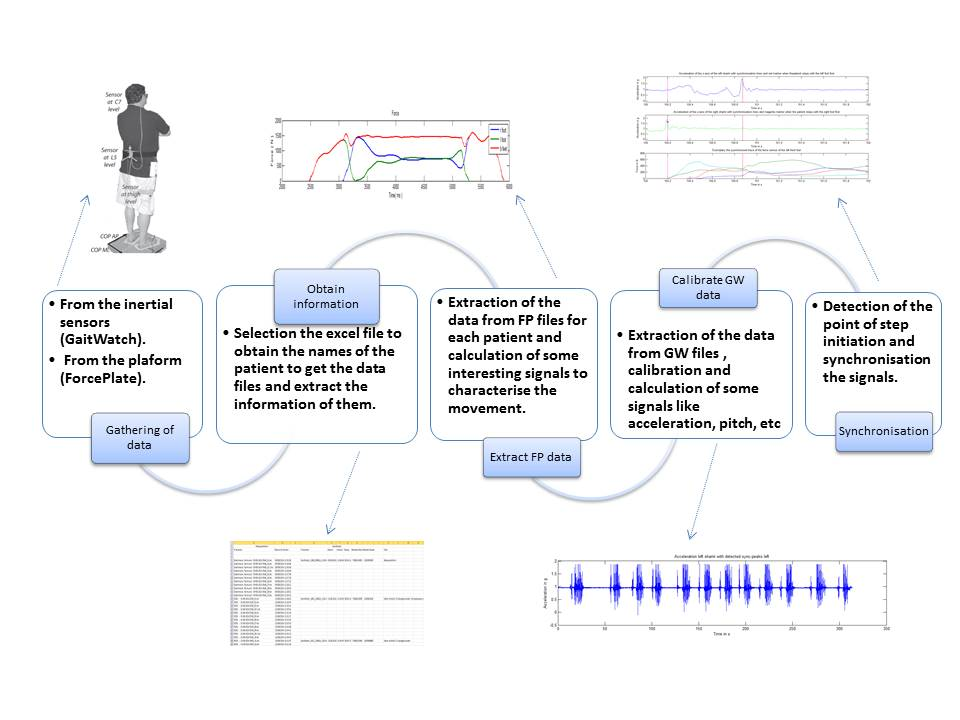
\epsfig{file=imagenes/diagramSynchronisation, width=8cm}
	\caption{Diagram of the Synchronisation's progress.}
	\label{fig:arte1}
\end{figure}

\subsection{Design of developed code  in Matlab}
\subsubsection{Selection, reading and obtaining of information from the excel file}
All patients data , that is, the different files have been generated after the gathering (  of the force plate as well as Gait Watch), gathering date, duration of the experiment and other observations are saved in a Excel file. 

In order to automate all as much as possible, the code is in charge of extraction of the necessary data (files names) to carry out the appropriate calculations for each patient. This is done once the Excel file has been selected, thus, it have to have a specific structure to be able to read the data correctly.

At the end of this fraction of code, we save all file names of both systems (force plate and Gait Watch) corresponding to each patient, in order to access and extract them posteriorly.

\subsubsection{Extraction of the forceplate data}
As we said before, the  force plate data files are recorded independently each others, that is, there is a *.txt file for each repeat.
Each file contains the force data of the toes and heels of both feet. It really realises a distribution of the sensors to cover these four segments. Every measure is obtained for each point of time according to the sample frequency. Also, this file contains the force data from each cell that is part of platform in each frame.

Once we recover this data, some parameters are calculated for the movement characterization carried out over the platform. 

\begin{itemize}
	\item \textbf{Midline}: it represents the midline between both feet. This is important to find the gap between feet and it gives us a idea of their position in the platform. Thus, we carry out the sum of cells force in the anterior-posterior direction. So, this line is in the minimum between two maximum corresponding to the position of both feet. We use this parameter to calculate the center of pressure.
	
	\item \textbf{The total force in the platform for each point of time}: This signal is useful to do the synchronisation due to we can determine clearer when the patient touches the plate.
	
	\item \textbf{Antero-posterior COP}: center of pressure forward-backward direction.
	
	\item \textbf{Medio-lateral  COP}: center of pressure  in right and left direction.
	
	
\end{itemize}

Center of pressure can be expressed as follows:

\begin{equation}
	\label{COP}
	R=\sum_{i}^{n}m_{i}r_{i}
\end{equation}


Where R is the “Center of pressure”, M is the total force and mi are the force that are located in space with coordinated ri, in this case, in the plane. This location (ri) is calculate with respect to the midline.

These signals help us to characterise Anticipatory Postural Adjustments  before gait.  APAs indicate the movement or swinging of body before walk or carry out some movement. Thus, these are the interesting  measures to compare between each repeat as well as each patients to characterise the movement, determine if there is a pattern and figure out the differences and similarities between them.

All these signals are saved for each cycle in a single variable corresponding to the patient.


\subsubsection{Calibration of the GaitWatch data}
When we are working with sensors, calibration is one of the most important aspect that needs to be carried out. Prior to the calibration process,
the information at the sensors  will be a signal composed of integer
numbers  or real numbers bounded into a range which is determined by the precision of the sensors and converters. These numeric values lack of physical value, so it is absolutely necessary to convert them into a scale that can be measured in physical units.

The sensors present several errors due to some effects like scale factor may not be linear or the triad isn’t perfectly orthogonal. To remove these undesired effects, the software include a model to compensate this before the calibration. 
To do so, we have used the code made by Dr. Alberto Olivares Vicente in his doctoral thesis, with minor modifications of his work.

Besides the unwanted effects mentioned above, the output of magnetometers is distorted by wide band measurement noise appearing several large peaks of noise in the signals. To remove this automatically, we used a threshold considering that these peaks are much greater than the mean of the signal.


The erroneus values in the magnetometer signal are removed sustituting these samples by the subsequent value unless the erroneous value is in the last position of the singal, in which case it is substituted by the preceding value.

\subsubsection{Synchronisation}	
\subsection{Results discurssion}


\section{APA analysis}

